% Figure from MATH 591 notes, section 67. After the board (Lecture 24): local existence on a manifold via a chart.
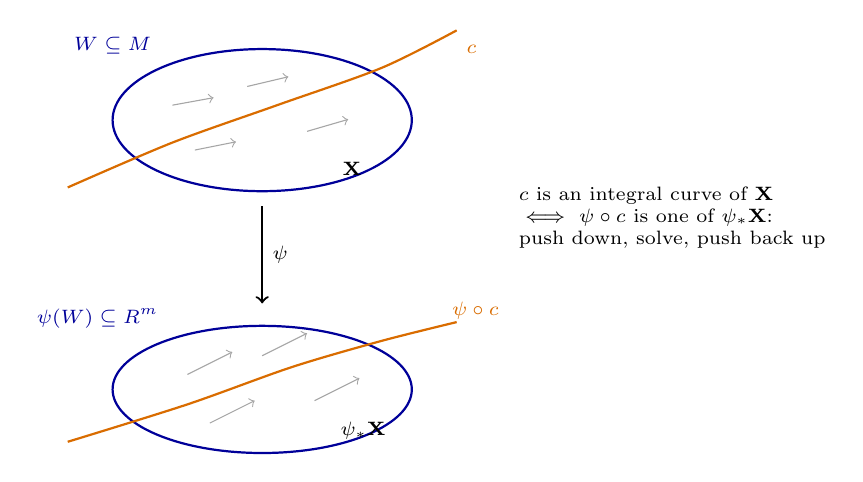
\begin{tikzpicture}[scale=0.95]
\draw[thick, blue!60!black] (0,3.7) ellipse (2.0 and 0.95); \node[blue!60!black, font=\scriptsize] at (-2.0,4.7) {$W \subseteq M$};
\draw[->, gray!70] (-1.20,3.90) -- (-0.65,4.00);
\draw[->, gray!70] (-0.20,4.15) -- (0.35,4.28);
\draw[->, gray!70] (0.60,3.55) -- (1.15,3.71);
\draw[->, gray!70] (-0.90,3.30) -- (-0.35,3.41);
\draw[orange!85!black, thick] plot[smooth] coordinates {(-2.6,2.8) (-1.2,3.4) (0.2,3.9) (1.6,4.4) (2.6,4.9)};
\node[orange!85!black, font=\scriptsize] at (2.8,4.65) {$c$}; \node[font=\scriptsize] at (1.2,3.05) {$\mathbf{X}$};
\draw[->, thick] (0,2.55) -- (0,1.25) node[midway, right, font=\scriptsize] {$\psi$};
\draw[thick, blue!60!black] (0,0.1) ellipse (2.0 and 0.85); \node[blue!60!black, font=\scriptsize] at (-2.2,1.05) {$\psi(W) \subseteq \mathbb{R}^m$};
\draw[->, gray!70] (-1.00,0.30) -- (-0.40,0.60);
\draw[->, gray!70] (0.00,0.55) -- (0.60,0.85);
\draw[->, gray!70] (0.70,-0.05) -- (1.30,0.25);
\draw[->, gray!70] (-0.70,-0.35) -- (-0.10,-0.05);
\draw[orange!85!black, thick] plot[smooth] coordinates {(-2.6,-0.6) (-1.0,-0.1) (0.4,0.4) (1.6,0.75) (2.6,1.0)};
\node[orange!85!black, font=\scriptsize] at (2.85,1.15) {$\psi \circ c$}; \node[font=\scriptsize] at (1.35,-0.45) {$\psi_*\mathbf{X}$};
\node[font=\scriptsize, anchor=west, align=left] at (3.3,2.4) {$c$ is an integral curve of $\mathbf{X}$\\ $\iff$ $\psi \circ c$ is one of $\psi_*\mathbf{X}$:\\ push down, solve, push back up};
\end{tikzpicture}
